\documentclass[utf8x, 14pt, bold, times]{G7-32} % Стиль (по умолчанию будет 14pt)

\sloppy

% Настройки стиля ГОСТ 7-32
% Для начала определяем, хотим мы или нет, чтобы рисунки и таблицы нумеровались в пределах раздела, или нам нужна сквозная нумерация.
%\EqInChapter % формулы будут нумероваться в пределах раздела
%\TableInChapter % таблицы будут нумероваться в пределах раздела
%\PicInChapter % рисунки будут нумероваться в пределах раздела

% Добавляем гипертекстовое оглавление в PDF
\usepackage[
bookmarks=true, colorlinks=true, unicode=true,
urlcolor=black,linkcolor=black, anchorcolor=black,
citecolor=black, menucolor=black, filecolor=black,
]{hyperref}

\AfterHyperrefFix

% полезный пакет для микротипографии, увы под xelatex мало чего умеет,
% но под pdflatex хорошо улучшает читаемость
\usepackage{microtype}

% Тире могут быть невидимы в Adobe Reader
\ifInvisibleDashes
\MakeDashesBold
\fi

\usepackage{graphicx}   % Пакет для включения рисунков

% С такими оно полями оно работает по-умолчанию:
% \RequirePackage[left=20mm,right=10mm,top=20mm,bottom=20mm,headsep=0pt,includefoot]{geometry}
% Если вас тошнит от поля в 10мм --- увеличивайте до 20-ти, ну и про переплёт не забывайте:

\geometry{right=10mm}
\geometry{left=30mm}
\geometry{top=20mm}
\geometry{bottom=20mm}
% считать от нижней границы текста
\geometry{ignorefoot}


% Пакет Tikz
\usepackage{tikz}
\usetikzlibrary{arrows,positioning,shadows}

% Произвольная нумерация списков.
\usepackage{enumerate}

% ячейки в несколько строчек
\usepackage{multirow}

% itemize внутри tabular
\usepackage{paralist,array}

%\setlength{\parskip}{1ex plus0.5ex minus0.5ex} % разрыв между абзацами
\setlength{\parskip}{1ex} % разрыв между абзацами
\usepackage{blindtext}

% Центрирование подписей к плавающим окружениям
%\usepackage[justification=centering]{caption}

\usepackage{newfloat}
\DeclareFloatingEnvironment[
placement={!ht},
name=Equation
]{eqndescNoIndent}
\edef\fixEqndesc{\noexpand\setlength{\noexpand\parindent}{\the\parindent}\noexpand\setlength{\noexpand\parskip}{\the\parskip}}
\newenvironment{eqndesc}[1][!ht]{%
    \begin{eqndescNoIndent}[#1]%
\fixEqndesc%
}
{\end{eqndescNoIndent}}

% Располагает все картинки (floats) до начала
% следующего раздела
\usepackage[section]{placeins}

% Двойная горизонтальная линия у таблиц
\usepackage{hhline}
% Расстояние между линиями
\setlength\doublerulesep{.5pt}

% Нумерация списка не по ГОСТУ.
% Первый уровень числа, второй - буквы
\renewcommand{\labelenumi}{\arabic{enumi})}
\renewcommand{\labelenumii}{\asbuk{enumii})}
\renewcommand{\labelitemi}{$\bullet$}

% Настройки листингов.
\usepackage{local-minted}

\usepackage{amsmath}
\makeatletter
\let\save@mathaccent\mathaccent
\newcommand*\if@single[3]{%
  \setbox0\hbox{${\mathaccent"0362{#1}}^H$}%
  \setbox2\hbox{${\mathaccent"0362{\kern0pt#1}}^H$}%
  \ifdim\ht0=\ht2 #3\else #2\fi
  }
%The bar will be moved to the right by a half of \macc@kerna, which is computed by amsmath:
\newcommand*\rel@kern[1]{\kern#1\dimexpr\macc@kerna}
%If there's a superscript following the bar, then no negative kern may follow the bar;
%an additional {} makes sure that the superscript is high enough in this case:
\newcommand*\widebar[1]{\@ifnextchar^{{\wide@bar{#1}{0}}}{\wide@bar{#1}{1}}}
%Use a separate algorithm for single symbols:
\newcommand*\wide@bar[2]{\if@single{#1}{\wide@bar@{#1}{#2}{1}}{\wide@bar@{#1}{#2}{2}}}
\newcommand*\wide@bar@[3]{%
  \begingroup
  \def\mathaccent##1##2{%
%Enable nesting of accents:
    \let\mathaccent\save@mathaccent
%If there's more than a single symbol, use the first character instead (see below):
    \if#32 \let\macc@nucleus\first@char \fi
%Determine the italic correction:
    \setbox\z@\hbox{$\macc@style{\macc@nucleus}_{}$}%
    \setbox\tw@\hbox{$\macc@style{\macc@nucleus}{}_{}$}%
    \dimen@\wd\tw@
    \advance\dimen@-\wd\z@
%Now \dimen@ is the italic correction of the symbol.
    \divide\dimen@ 3
    \@tempdima\wd\tw@
    \advance\@tempdima-\scriptspace
%Now \@tempdima is the width of the symbol.
    \divide\@tempdima 10
    \advance\dimen@-\@tempdima
%Now \dimen@ = (italic correction / 3) - (Breite / 10)
    \ifdim\dimen@>\z@ \dimen@0pt\fi
%The bar will be shortened in the case \dimen@<0 !
    \rel@kern{0.6}\kern-\dimen@
    \if#31
      \overline{\rel@kern{-0.6}\kern\dimen@\macc@nucleus\rel@kern{0.4}\kern\dimen@}%
      \advance\dimen@0.4\dimexpr\macc@kerna
%Place the combined final kern (-\dimen@) if it is >0 or if a superscript follows:
      \let\final@kern#2%
      \ifdim\dimen@<\z@ \let\final@kern1\fi
      \if\final@kern1 \kern-\dimen@\fi
    \else
      \overline{\rel@kern{-0.6}\kern\dimen@#1}%
    \fi
  }%
  \macc@depth\@ne
  \let\math@bgroup\@empty \let\math@egroup\macc@set@skewchar
  \mathsurround\z@ \frozen@everymath{\mathgroup\macc@group\relax}%
  \macc@set@skewchar\relax
  \let\mathaccentV\macc@nested@a
%The following initialises \macc@kerna and calls \mathaccent:
  \if#31
    \macc@nested@a\relax111{#1}%
  \else
%If the argument consists of more than one symbol, and if the first token is
%a letter, use that letter for the computations:
    \def\gobble@till@marker##1\endmarker{}%
    \futurelet\first@char\gobble@till@marker#1\endmarker
    \ifcat\noexpand\first@char A\else
      \def\first@char{}%
    \fi
    \macc@nested@a\relax111{\first@char}%
  \fi
  \endgroup
}
\makeatother


\begin{document}

\frontmatter % выключает нумерацию ВСЕГО; здесь начинаются ненумерованные главы: реферат, введение, глоссарий, сокращения и прочее.

\newcommand{\university}{
    Федеральное~государственное~автономное \\
    образовательное~учреждение \\
    высшего образования \\
    <<СИБИРСКИЙ~ФЕДЕРАЛЬНЫЙ~УНИВЕРСИТЕТ>>}
\newcommand{\faculty}{Институт~космических~и~информационных~технологий}
\newcommand{\department}{Кафедра~прикладной~математики~и~компьютерной~безопасности}
\newcommand{\city}{Красноярск}
\newcommand{\docname}{ОТЧЕТ~ПО~ЛАБОРАТОРНОЙ~РАБОТЕ}
\newcommand{\num}{~№1}
\newcommand{\topic}{Симметричная криптография. Простые шифры}
\newcommand{\variant}{Вариант~№~1}
\newcommand{\tutorname}{Ю.~В.~Потылицина}
\newcommand{\studentname}{С.~А.~Абрамов}
\newcommand{\group}{КИ20-08Б}
\newcommand{\gradebook}{032049480}

\renewcommand*{\maketitle}{
\begin{titlepage}
    \thispagestyle{empty}
    \begin{center}
        \university \\
        \faculty \\
		\department \\[6cm]

        \textbf{\docname \num} \\
		\topic \\
        \variant \\[5.1cm]

        \vfill
        \setlength\extrarowheight{-2pt}
        \begin{tabular*}{\textwidth}{@{\extracolsep{\fill}} lcl}
            \normalsize{Преподаватель:} & \underline{\hspace{3cm}} & \normalsize{\tutorname} \\
                          & {\small подпись, дата} & \\
            \normalsize{Студент:}~\normalsize{\group,~\gradebook}   & \underline{\hspace{3cm}} & \normalsize{\studentname} \\
                          & {\small подпись, дата} & \\
        \end{tabular*}
        \vfill
		\city~\the\year
	\end{center}
\end{titlepage}
}

\maketitle

\newpage
\tableofcontents

\nobreakingbeforechapters
%\breakingbeforechapters

\newpage
\Introduction

\textbf{Цель работы:}

\begin{itemize}
\item познакомиться с основами симметричного шифрования;
\item познакомиться с простыми симметричными криптографическими
      шифрами на основе методов подстановок, перестановок и гаммирования;
\item освоить основные этапы проектирования и реализации симметричных
      шифров.
\end{itemize}

\textbf{Задание на работу:}

\begin{itemize}
\item разработать и составить в виде блок-схемы алгоритмы шифрования и дешифрования текста
      на на основе <<магических>> квадратов размерностью $N \times N$;
\item убедиться в правильности составления алгоритмов и затем на языке
      программирования составить программу, которая реализует данные алгоритмы;
\item на ряде контрольных примеров (не менее 10) открытого текста, состоящего
      из различного количества символов, проверить правильность работы алгоритмов
      шифрования и дешифрования;
\item разработанная программа должна содержать графический интерфейс пользователя.
\end{itemize}


\mainmatter % это включает нумерацию глав и секций в документе ниже
\newpage

\chapter{Описание алгоритма}

\section{Алгоритм шифрования}

\begin{itemize}
\item Создать пустую строку $cipher$ для хранения зашифрованного текста;
\item Определить длину $l$ исходного текста;
\item Вычислить корень из длины текста и округлить вверх.
      Получим порядок квадрата $n = \lceil \sqrt{l} \rceil$; 
\item Сгенерировать магический квадрат порядка $n$;
\item Пройти по магическому квадрату сверху вниз ($i$ - номер строки),
      слева направо ($j$ - номер столбца). При этом, если значение
      $a_{i,j}$ меньше или равно длине сообщения ($a_{i,j} <= l$),
      добавить символ, стоящий в исходном тексте на месте $a_{i,j}-1$,
      в конец строки $cipher$. 
\end{itemize}

Блок-схема представлена на рисунке \ref{ris:magic-square-encrypt}.

\vspace{\baselineskip}
\begin{figure}[H]
\center{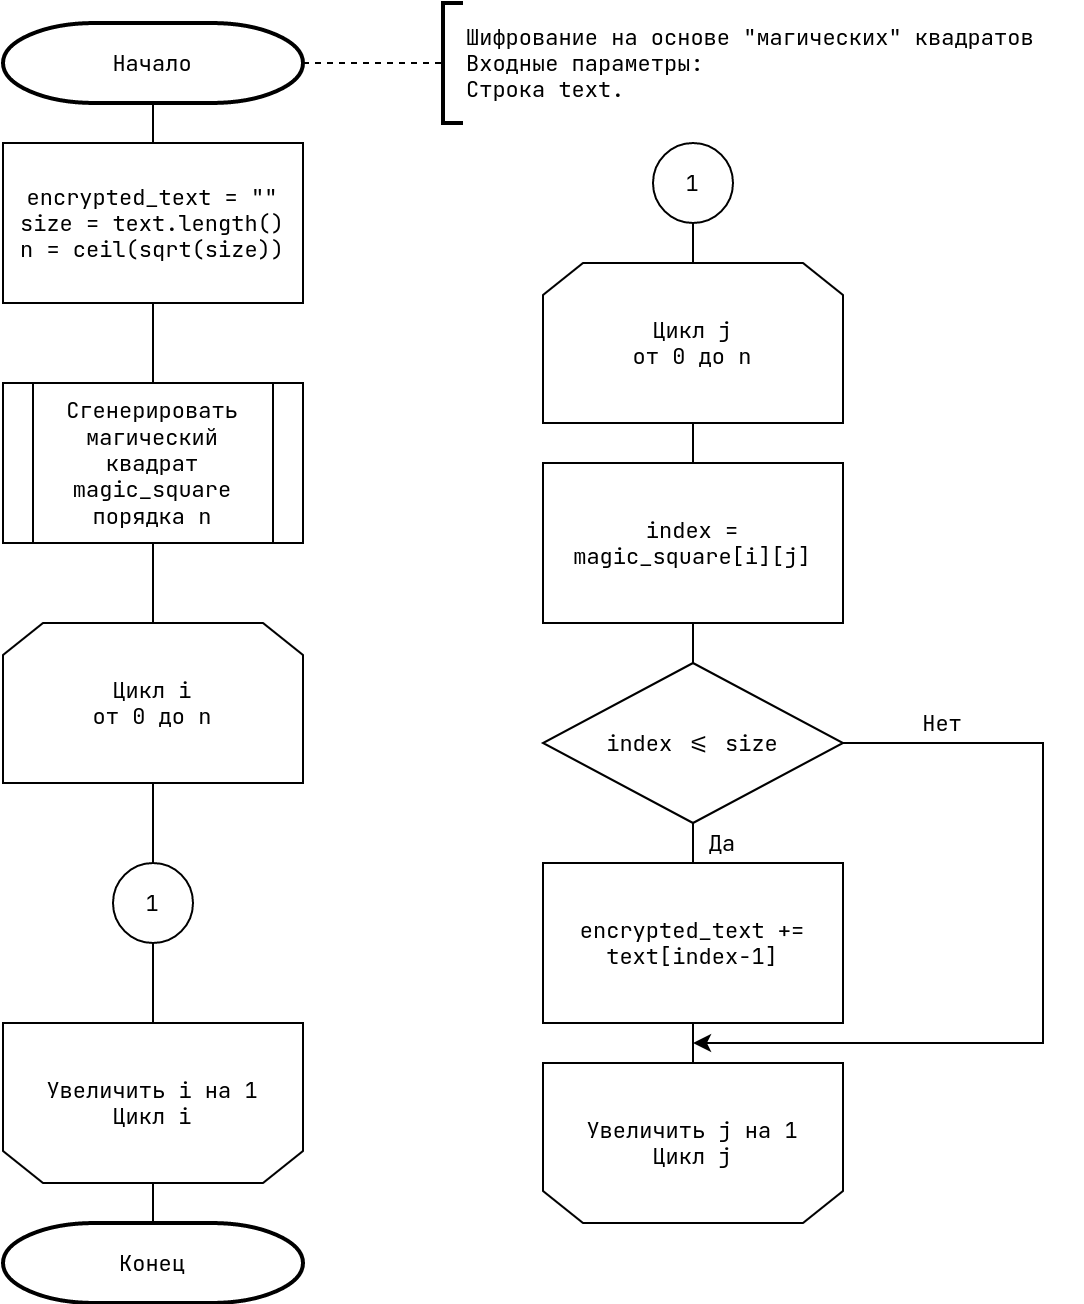
\includegraphics[width=0.5\linewidth]{figures/magic-square-encrypt}}
    \caption{Блок-схема алгоритма шифрования на основе <<магических>> квадратов}
\label{ris:magic-square-encrypt}
\end{figure}

\section{Алгоритм расшифрования}

\begin{itemize}
\item Определить длину $l$ зашифрованного текста;
\item Создать строку $text$ длиной $l$ для хранения расшифрованного текста,
      а также счетчик количества символов в строке $c=0$;
\item Вычислить корень из длины текста и округлить вверх.
      Получим порядок квадрата $n = \lceil \sqrt{l} \rceil$; 
\item Сгенерировать магический квадрат порядка $n$;
\item Пройти по магическому квадрату сверху вниз ($i$ - номер строки),
      слева направо ($j$ - номер столбца). При этом, если значение
      $a_{i,j}$ меньше или равно длине сообщения ($a_{i,j} <= l$),
      добавить символ, стоящий в зашифрованном тексте на месте $c$,
      в $text$ на место $a_{i,j}-1$. После этого увеличить $c$ на 1. 
\end{itemize}

Блок-схема представлена на рисунке \ref{ris:magic-square-decrypt}.

\vspace{\baselineskip}
\begin{figure}[H]
\center{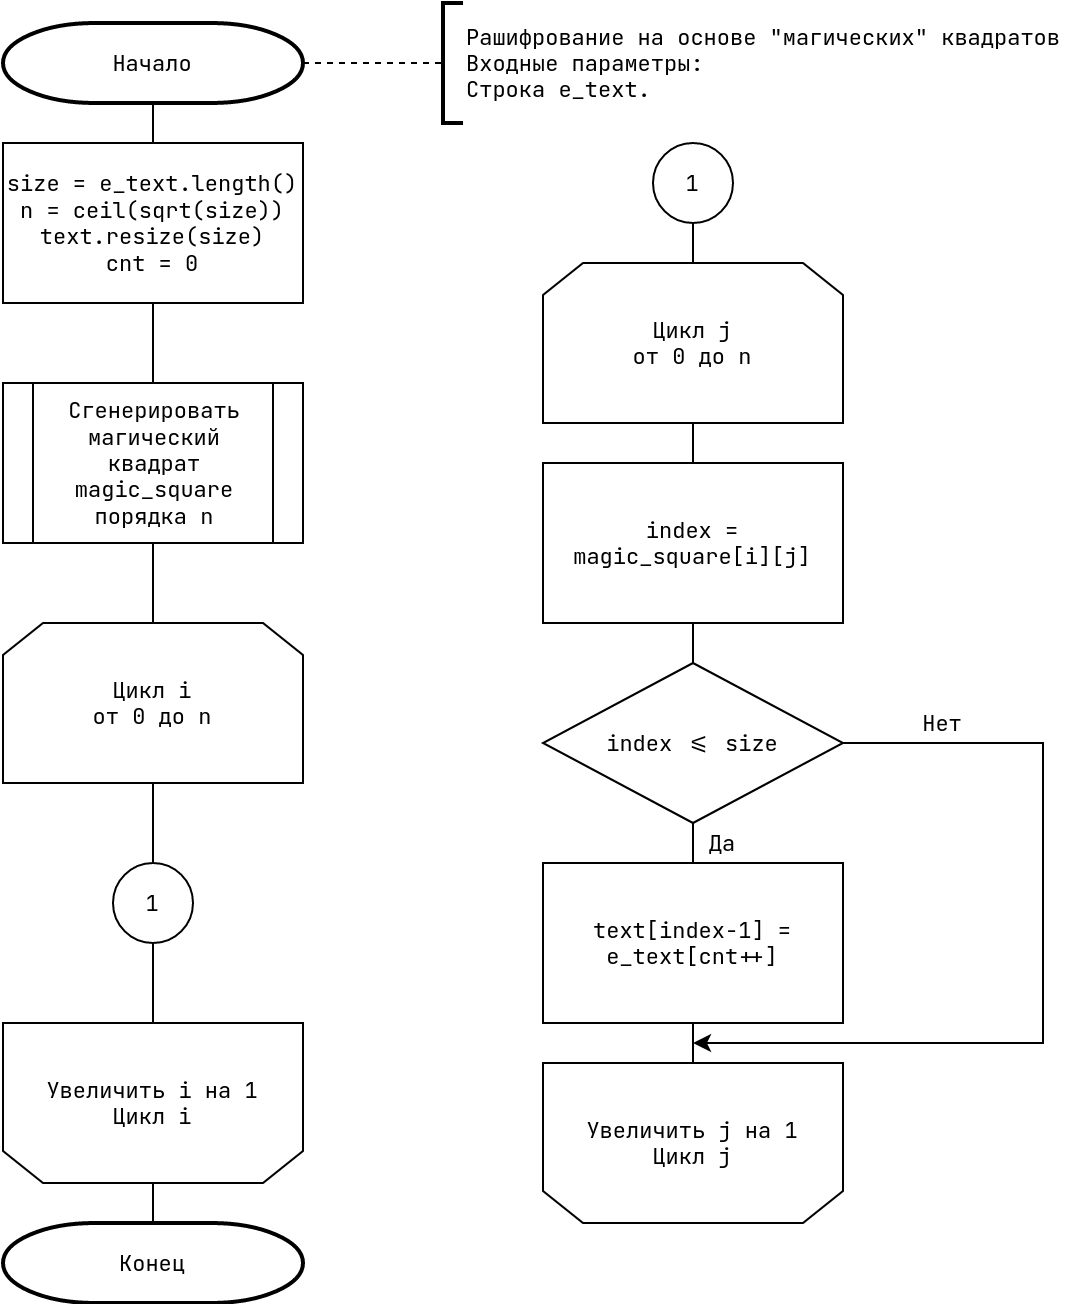
\includegraphics[width=0.5\linewidth]{figures/magic-square-decrypt}}
    \caption{Блок-схема алгоритма расшифрования на основе <<магических>> квадратов}
\label{ris:magic-square-decrypt}
\end{figure}

\chapter{Оценка алгоритма}

Легко определить и взломать частотным анализом. А также
для передачи ключа необходимо иметь защищенный канал связи.

\chapter{Примеры работы программы}

\section{Пример 1}

\textbf{Исходный текст:} \\
    Hello, World!

\textbf{Зашифрованный текст:} \\
    oleW! Hd,olrl

Результаты работы программы представлены на рисунках~\ref{ris:encode-test-1}-\ref{ris:decode-test-1}.

\vspace{\baselineskip}
\begin{figure}[H]
\center{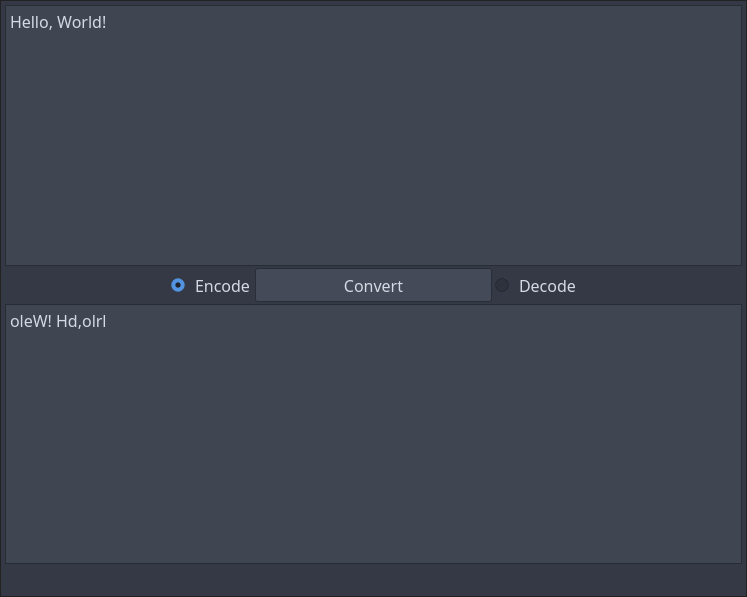
\includegraphics[width=0.7\linewidth]{figures/encode-test-1}}
    \caption{Шифрование}
\label{ris:encode-test-1}
\end{figure}

\vspace{\baselineskip}
\begin{figure}[H]
\center{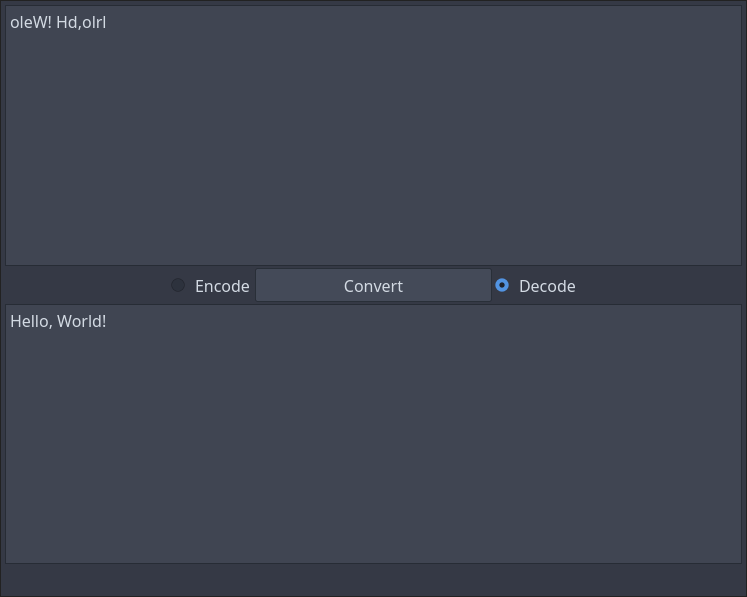
\includegraphics[width=0.7\linewidth]{figures/decode-test-1}}
    \caption{Расшифрование}
\label{ris:decode-test-1}
\end{figure}


\section{Пример 2}

\textbf{Исходный текст:} \\
    Привет, Мир!

\textbf{Зашифрованный текст:} \\
    Мир ,П!терив

Результаты работы программы представлены на рисунках~\ref{ris:encode-test-2}-\ref{ris:decode-test-2}.

\vspace{\baselineskip}
\begin{figure}[H]
\center{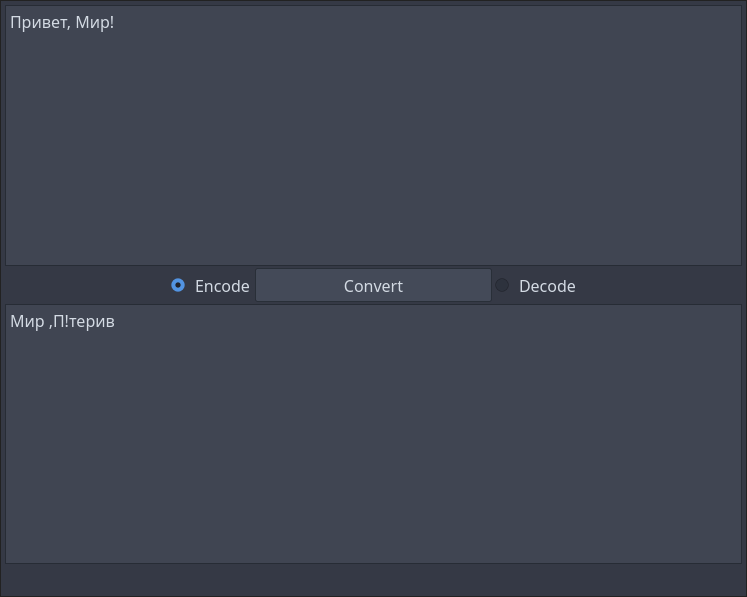
\includegraphics[width=0.7\linewidth]{figures/encode-test-2}}
    \caption{Шифрование}
\label{ris:encode-test-2}
\end{figure}

\vspace{\baselineskip}
\begin{figure}[H]
\center{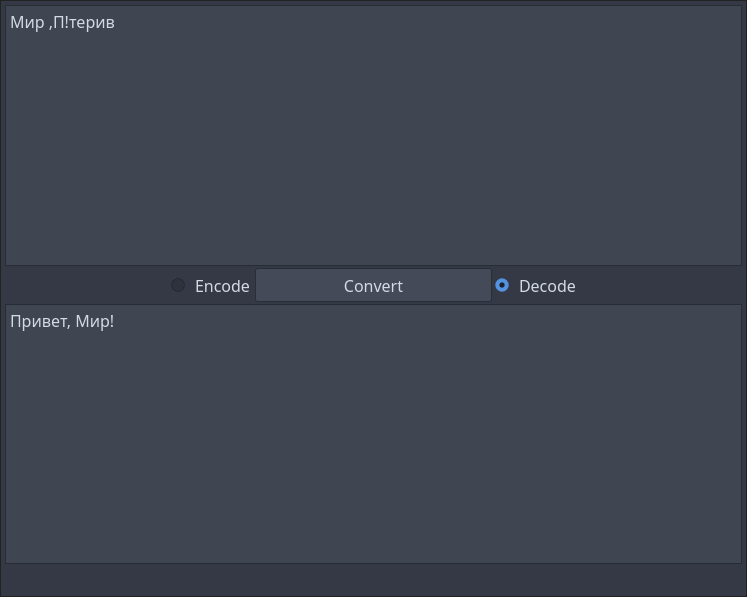
\includegraphics[width=0.7\linewidth]{figures/decode-test-2}}
    \caption{Расшифрование}
\label{ris:decode-test-2}
\end{figure}


\section{Пример 3}

\textbf{Исходный текст:} \\
    Шифром вертикальной перестановки называют популярную разновидность
    шифра маршрутной перестановки. В нем используется прямоугольник, в
    котором сообщение вписывается обычным способом (по строкам слева направо).
    Выписываются буквы по вертикали, а столбцы при этом берутся в порядке,
    определяемом ключом. Пусть, например, этот ключ таков: (5, 1, 4, 7, 2, 6, 3),
    и с его помощью надо зашифровать сообщение:

\textbf{Зашифрованный текст:} \\
    тосмВша тог тодрв с  я ррирре,эчяп о.ямр.а кеф 1 юроып) опимюввис ,лкпц
    оос к уо ш ,ре  бывптрваннмаи5(ммвлва(еоярраоз , ио окр атсоятр: 
    о):рмятупмвотнфсфеид3впессбаоыкеаилина оаят  нбс утшуеен,кнлуая оивзс прШщ
    6а ер сасп ьеьоепбю т,де,твов,лртп  ь, ьебиюеп коесотйо2чтр лалсеипп нюоощюспмавс
    инсийдансо уоокы мньл оивь м,л тисмыещомнвыльо7кПэтианчбгетозатп   ,рпкоыоунунака
    ,т.е ыВрбоо рзниво4омкие

Результаты работы программы представлены на рисунках~\ref{ris:encode-test-3}-\ref{ris:decode-test-3}.

\vspace{\baselineskip}
\begin{figure}[H]
\center{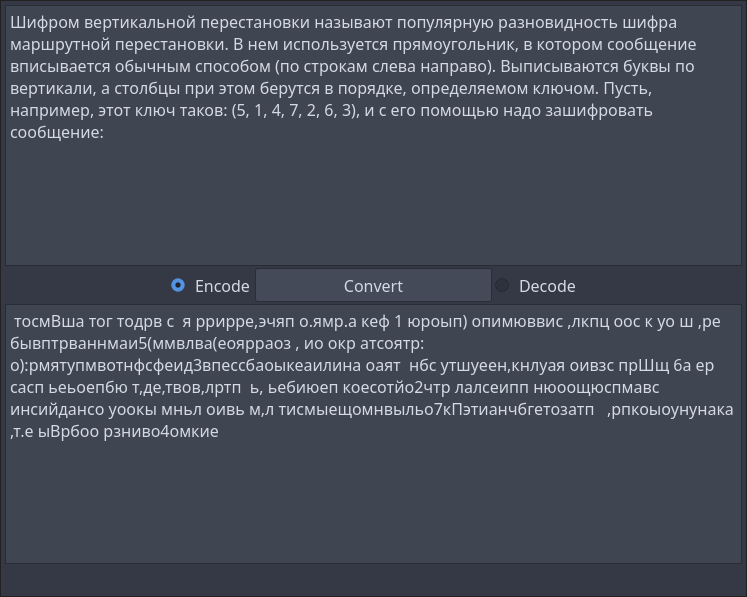
\includegraphics[width=0.7\linewidth]{figures/encode-test-3}}
    \caption{Шифрование}
\label{ris:encode-test-3}
\end{figure}

\vspace{\baselineskip}
\begin{figure}[H]
\center{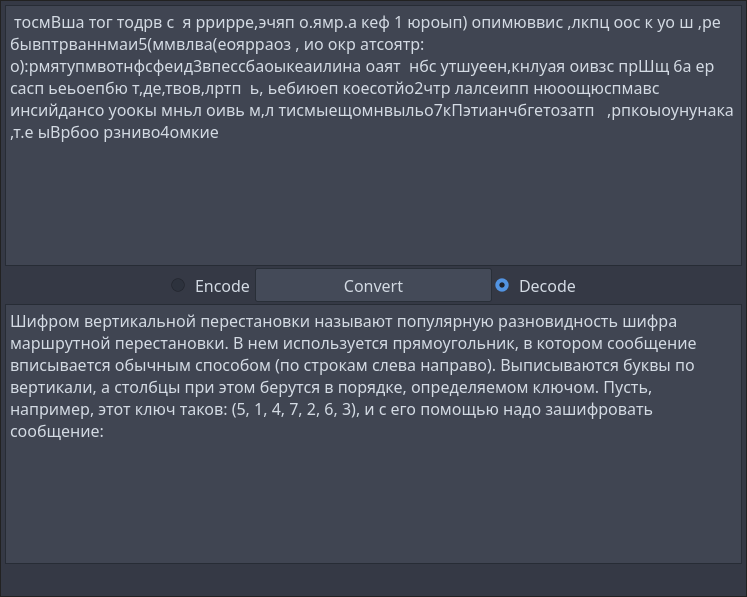
\includegraphics[width=0.7\linewidth]{figures/decode-test-3}}
    \caption{Расшифрование}
\label{ris:decode-test-3}
\end{figure}


\section{Пример 4}

\textbf{Исходный текст:} \\
    A magic square of order n is an arrangement of n\^~2 numbers,
    usually distinct integers, in a square, such that the n numbers
    in all rows, all columns, and both diagonals sum to the same constant.
    A magic square contains the integers from 1 to n\^~2. \\
    The constant sum in every row, column and diagonal is called the magic
    constant or magic sum, M. The magic constant of a normal magic square
    depends only on n and has the following value: M = n (n\^~2 + 1) / 2.

\textbf{Зашифрованный текст:} \\
    cgs orar aa2loamn ,we eb he,ru\^~o m asio ch ltgsrqnfsrets rettdl eras(
    dohTnl hninahte   enn  oayTig  cnbncnhepa.cnr
    ~aoauimai t e M oe.emt n u g= sdf cgv2h  ,isnsaMa o,iae\^~tAms  tim he
    mgi n  uns,c  : rtuadn s.smren2 edansm iont ueri\^~nAunua  d tinslbatn
    r.laqtcenm aalomus fe2a ssihau1ttacuqidodvn ngt s nsn ns   r  coa n
    monol nayto/ icmdmtocogla  ln  gn  eunr cai enlef)nogrllafe ed,hiamo1i
    aclot ram st ue  wymiocssruahw ,sge+ol g anoeqstotsunr lnlatc 

Результаты работы программы представлены на рисунках~\ref{ris:encode-test-4}-\ref{ris:decode-test-4}.

\vspace{\baselineskip}
\begin{figure}[H]
\center{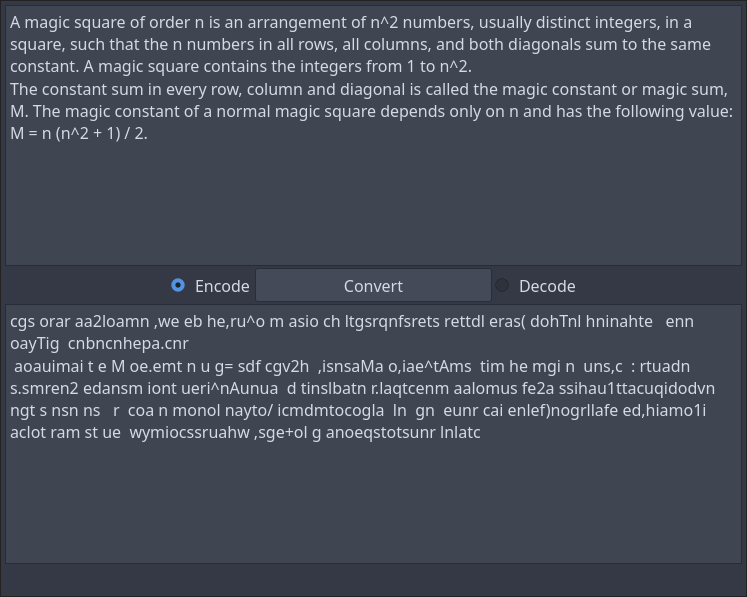
\includegraphics[width=0.7\linewidth]{figures/encode-test-4}}
    \caption{Шифрование}
\label{ris:encode-test-4}
\end{figure}

\vspace{\baselineskip}
\begin{figure}[H]
\center{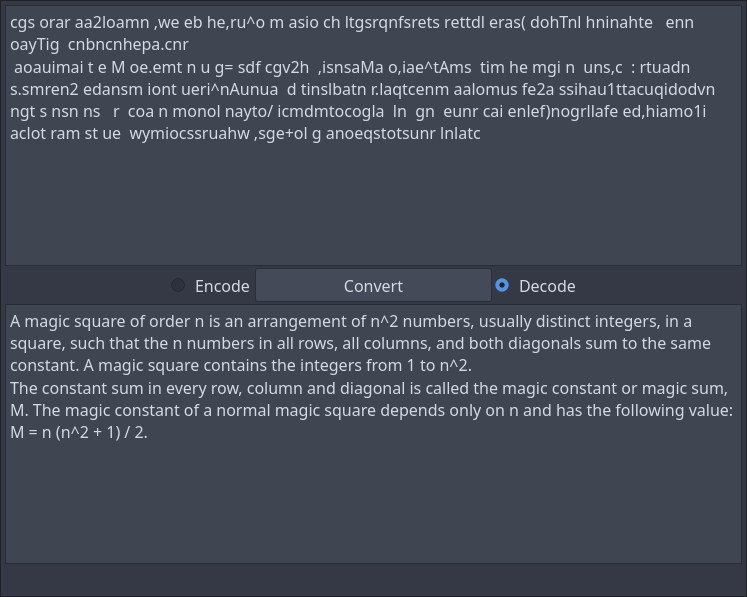
\includegraphics[width=0.7\linewidth]{figures/decode-test-4}}
    \caption{Расшифрование}
\label{ris:decode-test-4}
\end{figure}


\section{Пример 5}

\textbf{Исходный текст:} \\
    Настоящий стандарт университета устанавливает общие требования к построению,
    изложению и оформлению учебных документов, выполняемых студентами в процессе
    их обучения в университете.

\textbf{Зашифрованный текст:} \\
    биеблеиуеев  оеввщ сду,ерраиявсетвчютнно яцсоуитаут.еио т нс  стнрхнюеоетаеепыеижписттч 
    ммно щурНиувеуелкб адсб яклз оатнроиномия теа млдр инеттеао о,юааисвхпхфоиввс иитын ноирйн ны

Результаты работы программы представлены на рисунках~\ref{ris:encode-test-5}-\ref{ris:decode-test-5}.

\vspace{\baselineskip}
\begin{figure}[H]
\center{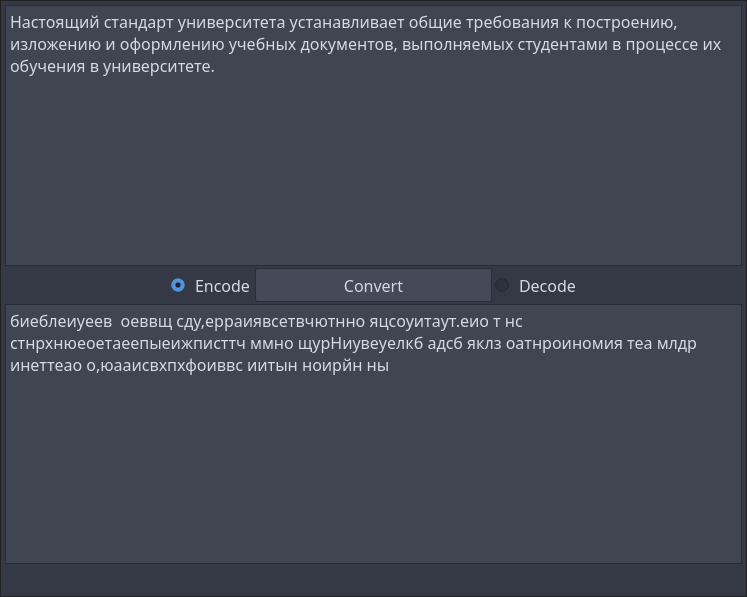
\includegraphics[width=0.7\linewidth]{figures/encode-test-5}}
    \caption{Шифрование}
\label{ris:encode-test-5}
\end{figure}

\vspace{\baselineskip}
\begin{figure}[H]
\center{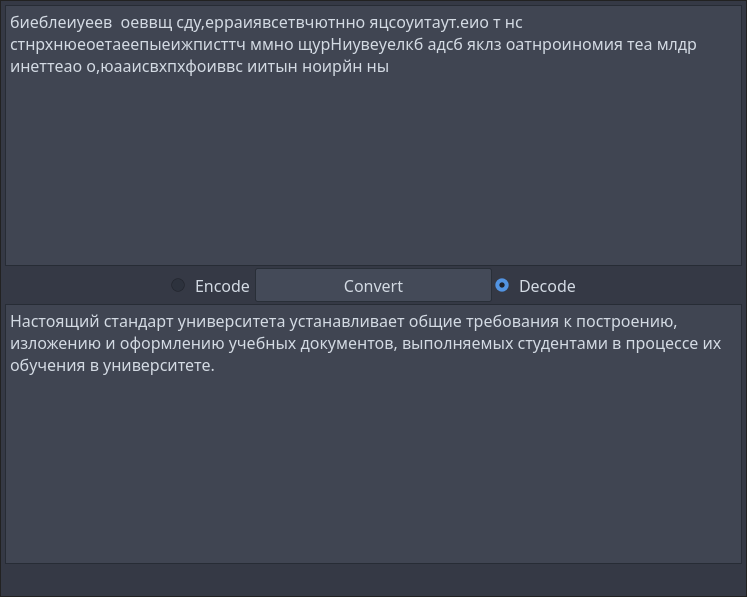
\includegraphics[width=0.7\linewidth]{figures/decode-test-5}}
    \caption{Расшифрование}
\label{ris:decode-test-5}
\end{figure}


\chapter{Исходный код}

\section{textencryptor.h}

\inputminted[fontsize=\footnotesize, breaklines]{cpp}{../../src/textencryptor.h}

\section{textencryptor.cpp}

\inputminted[fontsize=\footnotesize, breaklines]{cpp}{../../src/textencryptor.cpp}

\section{mainwindow.h}

\inputminted[fontsize=\footnotesize, breaklines]{cpp}{../../src/mainwindow.h}

\section{mainwindow.cpp}

\inputminted[fontsize=\footnotesize, breaklines]{cpp}{../../src/mainwindow.cpp}

\section{magicsquare.h}

\inputminted[fontsize=\footnotesize, breaklines]{cpp}{../../src/magicsquare.h}

\section{magicsquare.cpp}

\inputminted[fontsize=\footnotesize, breaklines]{cpp}{../../src/magicsquare.cpp}

\backmatter %% Здесь заканчивается нумерованная часть документа и начинаются ссылки и

\newpage
\Conclusion

В ходе работы изучил простые симметричные шифры на основе методов подстановок
и перестановок, а также их недостатки и преимущества. 

\end{document}
